%----------------------------------------------------------------------------
\chapter{Elméleti bevezetés}\label{ch:elmelet}
%----------------------------------------------------------------------------

Ezt a fejezetet a feladat értelmezésével fogom kezdeni, majd az alkalmazott matematikai hátteret mutatom be. Rövid lineáris algebrai bevezető után a háromdimenziós tér alapvető transzformációit tárgyalom. A fejezetet a lyukkamera-modell leírásával zárom.

%----------------------------------------------------------------------------
\section{Feladat értelmezése}
%----------------------------------------------------------------------------

A feladatom egy legalább két fix telepítésű kamerából álló kamerarendszer által megfigyelt térrészben egy tetszőleges pontban és irányban látható kép valós idejű helyreállíthatóságának vizsgálata, a probléma megoldhatósági korlátainak meghatározása, és egy megvalósítási terv készítése.

A dolgozat során két eltérő módszert mutatok be; a sztereó-kamerák és az optikai folyamok módszerét. Ezek közül az utóbbit implementálom, tesztelem és végül értékelem. A probléma megoldása során a könnyebb objektum-detektálás érdekében felteszem, hogy a rekonstruálandó objektumok mozognak a kamerák képein. Ez a kényszer igazodik a feladat kitűzésem második pontjához, és ennek így a tervezett megoldásom eleget tud tenni. A látott kép helyreállítása alatt az adott nézőpontból látható mozgó objektumok felismerését és azok kontúrjainak kirajzolását értem.

A valós idejű helyreállítóság vizsgálatát és az eredmények dokumentációját a következőknek megfelelően végzem el. Először egy darab mozgó objektumot fogok rekonstruálni, közben a nézőpontot beviteli vezérlők segítségével szabadon választhatjuk. Ezt követően két darab, lényegesen eltérő textúrával rendelkező mozgó objektumot helyezek a térrészbe, és vetem alá a helyreállításnak. Rekonstrukció során a feldolgozás sebességét az egységnyi idő alatt rekonstruált és kirajzolt képkockák számában határozom meg (FPS - \textit{frames per second}). Az eredmény minőségét, azaz a helyreállítás helyességét -- referencia rekonstrukció hiányában -- szubjektíven fogom értékelni.

A fejezet hátralévő részében a matematikai hátteret és a lyukkamera-modellt mutatom be.

%----------------------------------------------------------------------------
\section{Lineáris transzformációk}
%----------------------------------------------------------------------------

Legyen $B = \{\mathbf{b_1}, \mathbf{b_2}, \ldots, \mathbf{b_n}\}$ bázis $\mathbb{R}^n$-ben. Ekkor egy teszőleges $\mathbf{v} \in \mathbb{R}^n$ egyértelműen felírható a bázisvektorok lineáris kombinációjaként:

\[\mathbf{v} = \lambda_1\mathbf{b_1} + \lambda_2\mathbf{b_2} \ldots + \lambda_n\mathbf{b_n} \qquad \hbox{ahol }\lambda_i \in \mathbb{R}\]

Ekkor $\mathbf{v}$ koordinátái a $B$ bázisban:

\[[\mathbf{v}]_B = \left(\begin{array}{c} \lambda_1\\ \lambda_2\\ \vdots\\ \lambda_n\end{array}\right)\]

$\mathcal{F}: \mathbb{R}^n \rightarrow \mathbb{R}^n$ lineáris transzformáció, amennyiben tetszőleges $\mathbf{v}, \mathbf{w} \in \mathbb{R}^n$ és $\lambda \in \mathbb{R}$-re teljesül az alábbi:

\[\mathcal{F}(\mathbf{v} + \mathbf{w}) = \mathcal{F}(\mathbf{v}) + \mathcal{F}(\mathbf{w}) \quad \hbox{ és } \quad \mathcal{F}(\lambda\mathbf{v}) = \lambda\mathcal{F}(\mathbf{v})\]

Az $M$ mátrixot az $\mathcal{F}$  lineáris transzformáció mátrixának hívjuk $B$-ben, ha minden $\mathbf{v}\in \mathbb{R}^n$-re teljesül, hogy:

\[[\mathcal{F}(\mathbf{v})]_B = M \cdot [\mathbf{v}]_B\]

%----------------------------------------------------------------------------
\section{Affin transzformációk}
%----------------------------------------------------------------------------

Az $\sigma$ síkon vett affin transzformáción egy olyan $\phi : \sigma \rightarrow \sigma$ bijekciót értünk, amely minden $e\in\sigma$ egyenest $e'\in\sigma$ egyenesbe képez le. A lineáris algebra eszközeinek felhasználásával, egy tetszőleges $P(x, y)$ pont $P'(x', y')$ affin képe felírható az alábbi mátrix-egyenlettel:

\[\left(\begin{array}{c}x' \\y'\end{array}\right) = \left(\begin{array}{cc}a_{11} & a_{12}\\a_{21} & a_{22}\\\end{array}\right) \cdot \left(\begin{array}{c}x \\y\end{array}\right) + \left(\begin{array}{c}b_1 \\b_2\end{array}\right) \qquad \hbox{ahol} \qquad  \left|\begin{array}{cc}a_{11} & a_{12}\\a_{21} & a_{22}\\\end{array}\right| \neq 0\]

Vagyis egy affin transzformáció leírható egy lineáris transzformáció és egy eltolás egymásutánjával. Homogenizált alakban -- azaz a pontokat homogén koordinátarendszerben felírva -- az alábbi formát ölti:

\[\left(\begin{array}{c}x' \\y'\\ 1\end{array}\right) = \left(\begin{array}{ccc}a_{11} & a_{12} & b_1\\a_{21} & a_{22} & b_2\\0 & 0 & 1\end{array}\right) \cdot \left(\begin{array}{c}x \\ y\\ 1\end{array}\right)\]

%----------------------------------------------------------------------------
\section{A háromdimenziós tér alapvető transzformációi}
%----------------------------------------------------------------------------

A következőkben 4 alapvető affin transzformáció kerül bemutatásra a térben, ezek sorrendben: eltolás, forgatás, skálázás és nyírás.

\subsection{Eltolás}

Legyen $\mathbf{v}(v_x, v_y, v_z), \mathbf{t}(t_x, t_y, t_z)\in\mathbb{R}^3$, ekkor $\mathbf{v}$ vektor $\mathbf{t}$ eltoltja:

\[\left(\begin{array}{c}v_x' \\v_y'\\ v_z'\\ 1 \end{array}\right) = \left(\begin{array}{cccc}1 & 0 & 0 & t_x\\0 & 1 & 0 & t_y\\ 0 & 0 & 1 & t_z\\ 0 & 0 & 0 & 1\end{array}\right) \cdot \left(\begin{array}{c}v_x \\v_y\\ v_z\\ 1 \end{array}\right)\]

\subsection{Forgatás}

Legyen $\mathbf{v}(v_x, v_y, v_z)\in\mathbb{R}^3$ és $\theta\in\mathbb{R}$, ekkor $\mathbf{v}$ vektor $x$ tengely körüli $\theta$ szöggel való (jobb-kéz szabályt használva) elforgatottja:

\[\left(\begin{array}{c}v_x' \\v_y' \\v_z' \\ 1 \end{array}\right) = \left(\begin{array}{cccc}1 & 0 & 0 & 0\\0 & \cos (\theta) & -\sin (\theta) & 0\\ 0 & \sin(\theta) & \cos(\theta) & 0 \\ 0 & 0 & 0 & 1\end{array}\right) \cdot \left(\begin{array}{c}v_x\\ v_y\\ v_z\\ 1\end{array}\right)\]

\subsection{Skálázás}

Legyen $\mathbf{v}(v_x, v_y, v_z), \mathbf{s}(s_x, s_y, s_z)\in\mathbb{R}^3$, ekkor $\mathbf{v}$ vektor origóból történő skálázása $\mathbf{s}$-sel:

\[\left(\begin{array}{c}v_x' \\v_y' \\v_z' \\ 1 \end{array}\right) = \left(\begin{array}{cccc}s_x & 0 & 0 & 0\\0 & s_y & 0 & 0\\ 0 & 0 & s_z & 0\\ 0 & 0 & 0 & 1\end{array}\right) \cdot \left(\begin{array}{c}v_x\\ v_y\\ v_z\\ 1\end{array}\right)\]

\subsection{Nyírás}

A térbeli nyírás a tér $P$ pontjainak egy fix síkkal történő párhuzamos csúsztatása. Legyen $\mathbf{v}(v_x, v_y, v_z)\in\mathbb{R}^3$ és $\lambda\in\mathbb{R}$, ekkor a $\mathbf{v}$ vektor $x$ tengely irányában az $x-y$ sík mentén vett nyírása:

\[\left(\begin{array}{c}v_x' \\v_y' \\v_z' \\ 1 \end{array}\right) = \left(\begin{array}{cccc}1 & \lambda & 0 & 0\\0 & 1 & 0 & 0\\ 0 & 0 & 1 & 0\\ 0 & 0 & 0 & 1\end{array}\right) \cdot \left(\begin{array}{c}v_x\\ v_y\\ v_z\\ 1\end{array}\right) = \left(\begin{array}{c}v_x + \lambda\cdot v_y\\ v_y\\ v_z\\ 1\end{array}\right)\]

\subsection{Transzformációk egymásutánja}

Ha egy $\mathcal{A}_1, \mathcal{A}_2, \ldots, \mathcal{A}_n$ transzformáció sorozatnak megfelelő transzformációs mátrixok rendre $T_1, T_2, \ldots, T_n$, akkor $\mathbf{v}$ transzformáltja:
\[\mathbf{v}' = \mathcal{A}_n(\mathcal{A}_{n-1}(\ldots \mathcal{A}_2(\mathcal{A}_1(\mathbf{v}))\ldots)) = T_n \cdot T_{n-1} \cdot \ldots \cdot T_2 \cdot T_1 \cdot \mathbf{v}\]
Így az eredő transzformációt lényegében úgy kapjuk, hogy a transzformációs mátrixok szorzatával, azaz az ,,eredő transzformációs mátrixszal'' szorozzuk be a vektort:
\[\mathbf{v}' = T \cdot \mathbf{v} \qquad \hbox{ahol} \; T = \prod_{i=1}^{n}{T_i}\]

%----------------------------------------------------------------------------
\section{Perspektivikus projekció -- A lyukkamera-modell \label{sec:pinhole}}
%----------------------------------------------------------------------------

A kamerák a valós világot képezik le egy adott nézőpontból. A lyukkamera-modell alkalmazása során ezt a leképezést egy perspektivikus projekciónak tekintjük \cite[2.2. fejezet]{pinhole-model} (lásd \aref{fig:pinhole}. ábrát). A projekció középpontját (ahol az egyenesek metszik egymást) \textit{optikai középpontnak} ($C$) vagy \textit{kamera középpontnak}, az egyenest, ami merőleges a képsíkra, és átmegy az optikai középponton \textit{optikai tengelynek}, magát a metszéspontot ($P$) pedig \textit{főpontnak} nevezzük.

\begin{figure}[tbh]
\centering
\tdplotsetmaincoords{60}{130}
\begin{tikzpicture}[line join = round, line cap = round, >=triangle 45, tdplot_main_coords]
  
  \coordinate (O) at (0, 0, 0);
  
  % kocka
  
  \coordinate (C1) at (-4.5, -2, 1);
  \coordinate (C2) at (-4.5, -1, 1);
  \coordinate (C3) at (-4.5, -1, 2);
  \coordinate (C4) at (-4.5, -2, 2);
  \coordinate (C1B) at (-5, -2, 1);
  \coordinate (C2B) at (-5, -1, 1);
  \coordinate (C3B) at (-5, -1, 2);
  \coordinate (C4B) at (-5, -2, 2);
    \node [below right] at (C2) {\small $(X, Y, Z)$};

  \draw [dashed] (C1) -- (C2);
  \draw [dashed] (C2) -- (C3);
  \draw [dashed] (C3) -- (C4);
  \draw [dashed] (C4) -- (C1);
  \draw [dashed] (C1) -- (C1B);
  \draw [dashed] (C2) -- (C2B);
  \draw [dashed] (C3) -- (C3B);
  \draw [dashed] (C4) -- (C4B);
  \draw [dashed] (C1B) -- (C2B);
  \draw [dashed] (C2B) -- (C3B);
  \draw [dashed] (C3B) -- (C4B);
  \draw [dashed] (C4B) -- (C1B);
  
  
  % képsík
  
  \coordinate (I1) at (0, 0, 0);
  \coordinate (I1T) at (-0.5, -0.25, -0.15);
  \coordinate (I2) at (0, 5, 0);
  \coordinate (I2T) at (-0.5, 5.25, -0.15);
  \coordinate (I3) at (0, 5, 3);
  \coordinate (I3T) at (-0.5, 5.25, 3.15);
  \coordinate (I4) at (0, 0, 3);
  \coordinate (I4T) at (-0.5, -0.25, 3.15);
  
  \draw (I1) -- (I2);
  \draw (I2) -- (I3);
  \draw (I3) -- (I4);
  \draw (I4) -- (I1);

  \coordinate (UV) at (0.25, 0.75, 1.25);
  \node [cross] at (UV) {};
  \node [below right] at (UV) {\small $(u, v)$};

  % optikai tengely
  \coordinate (P) at (0, 2.5, 1.5);
  \coordinate (C) at (5, 2.5, 1.5);
  \coordinate (A) at (-1, 2.5, 1.5);

  \node [below] at (C) {\small $C$};
  \draw (C) -- (P);
  \node [cross] at (P) {};
  \node [below right] at (P) {\small $P$};
  \draw [dashed,-latex] (P) -- (A);
  
  % leképezés
  
  \draw [dotted] (C) -- (C2);
  
  % leképezés kerete
  
  \draw [black!15] (C) -- (I1T);
  \draw [black!15] (C) -- (I2T);
  \draw [black!15] (C) -- (I3T);
  \draw [black!15] (C) -- (I4T);
  
\end{tikzpicture}
\caption{Lyukkamera-modell, $(X, Y, Z)$ pont képe a képsíkon $(u, v)$ \label{fig:pinhole}}
\end{figure}

Tegyük fel, hogy az optikai tengely párhuzamos a $z$ tengellyel, és az optikai középpont a 3D-s koordinátarendszer origójában van. Ekkor az alábbi egyenlettel írható fel a projekció:

\[s \left(\begin{array}{c}
u \\ 
v \\
1
\end{array}\right) = \left(\begin{array}{cccc}
f & 0 & 0 & 0 \\ 
0 & f & 0 & 0\\
0 & 0 & 1 & 0
\end{array}\right) \left(\begin{array}{c}
X \\ 
Y \\
Z \\
1
\end{array}\right)\]

ahol $f$ a fókusztávolság ($C$ és a képsík távolsága), $s = Z$ pedig a skálázási tényező.

A manapság használt képalkotó rendszerek a képsík origójának nem a főpontot, hanem a kép balfelső sarkát tekintik, így a fenti egyenlet a következő  alakot ölti, amennyiben a főpont koordinátája $(o_x, o_y)$:

\[s \left(\begin{array}{c}
u \\ 
v \\
1
\end{array}\right) = \left(\begin{array}{cccc}
f & 0 & o_x & 0 \\ 
0 & f & o_y & 0 \\
0 & 0 & 1 & 0
\end{array}\right) \left(\begin{array}{c}
X \\ 
Y \\
Z \\
1
\end{array}\right)\]

Valódi kamerák használata esetén számolni kell azzal, hogy a lencséknek van radiális (lásd \aref{fig:radial-distortion}. ábra) és tangenciális torzításuk (ami abból adódik, hogy a lencse és a képalkotó sík nem párhuzamos). Mivel ezek csak a konkrét kamerától függnek, ezért mértékük kalibrációval meghatározható és hatásuk kiküszöbölhető. 

\begin{figure}[tbh]
\centering
\begin{subfigure}[b]{.32\linewidth}
	\centering
	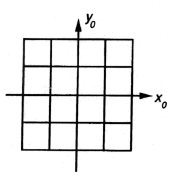
\includegraphics{figures/dist-1.png}
	\caption{Ideális eset}
  \end{subfigure}
\begin{subfigure}[b]{.32\linewidth}
	\centering
	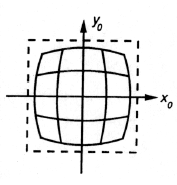
\includegraphics{figures/dist-2.png}
	\caption{,,Hordó-torzítás''}
  \end{subfigure}
\begin{subfigure}[b]{.32\linewidth}
	\centering
	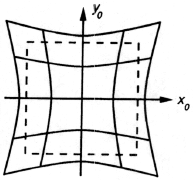
\includegraphics{figures/dist-3.png}
	\caption{,,Tűpárna-torzítás''}
  \end{subfigure}
\caption{Lencsék radiális torzítása \cite{distortion} \label{fig:radial-distortion}}
\end{figure}

A gyakorlatban gyakran használt modell, hogy a radiális torzítás esetében a torzított és a javított pontok között egy polinomfüggvény teremt kapcsolatot:

\[\left(\begin{array}{c}x_{\hbox{\small jav}}\\ y_{\hbox{\small jav}}\end{array}\right) = (1 + k_1r^2 + k_2r^4 + k_3r^6) \left(\begin{array}{c}x\\y\end{array}\right)\]

ahol $(x,y)$ volt az eredeti kép egy pixelének koordinátája, és $(x_{\hbox{\small jav}}, y_{\hbox{\small jav}})$ pedig az új koordináta a korrigált képen. Tangenciális torzítás pedig a következő egyenletek segítségével javítható:
\[x_{\hbox{\small jav}} = x + \Big(2p_1xy + p_2(r^2+2x^2)\Big)\]
\[y_{\hbox{\small jav}} = y + \Big(p_1(r^2+2y^2) + 2p_2xy\Big)\]
Ekkor $k_1, k_2$ és $k_3$ a radiális, $p_1$ és $p_2$ pedig a tangenciális torzítás együtthatói.

Kalibrálás során ezeket az együtthatókat határozzuk meg. A képen szereplő egyenesek görbületét, mint költség-függvényt, minimalizálva kiszámolhatjuk a radiális torzítást, hiszen ideális esetben nincs görbület. A gyakorlatban ez úgy történik, hogy egy előre ismert objektumot -- például egy sakktáblát -- detektálunk a képeken (lásd \aref{fig:chessboards}. ábra), és a sarokpontokat összekötő egyeneseket vizsgáljuk.

\begin{figure}[tbh]
\centering
\begin{subfigure}[b]{0.49\linewidth}
	\centering
	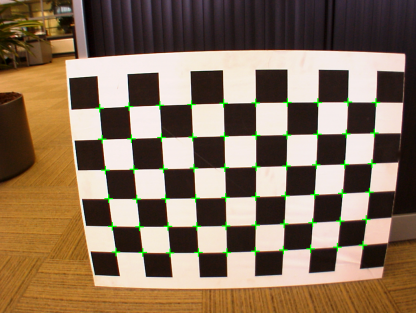
\includegraphics[width=200pt]{figures/distorted.png}
	\caption{Kamera képe, sarokpontokkal}
  \end{subfigure}
\begin{subfigure}[b]{0.49\linewidth}
	\centering
	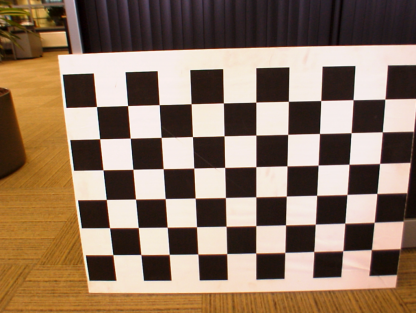
\includegraphics[width=200pt]{figures/undistorted.png}
	\caption{Javított kép}
  \end{subfigure}
\caption{Radiális torzítás meghatározása \cite{pinhole-model} \label{fig:chessboards}}
\end{figure}

Az előzőekben a kamera \textit{belső paramétereit} vizsgáltuk, melyeket a kamera lencséi és fókusztávolsága határoznak meg. Azonban szükséges beszélnük a \textit{külső paraméterekről} is, amely a kamera pozícióját és irányát mutatja a világ-koordinátához képest.

A gyakorlatban a kamera helyét és irányát egy $\mathbf{c} = (c_1, c_2, c_3)^T$ vektorral és egy $\mathbf{R}$ forgatási mátrixszal adjuk meg. Így ahhoz, hogy egy 3D-s pont képét megkapjuk, először a kamerát el kell tolni a világkoordináta-rendszer origójába, majd forgatni, vagyis:

\[s \left(\begin{array}{c}
u \\ 
v \\
1
\end{array}\right) = \left(\begin{array}{cccc}
f & 0 & o_x & 0 \\ 
0 & f & o_y & 0 \\
0 & 0 & 1 & 0
\end{array}\right) \left(\begin{array}{cccc}
r_{11} & r_{12} & r_{13} & 0 \\ 
r_{21} & r_{22} & r_{23} & 0 \\ 
r_{31} & r_{32} & r_{33} & 0 \\ 
0 & 0 & 0 & 1 \\ 
\end{array}\right) \left(\begin{array}{cccc}
1 & 0 & 0 & -c_1 \\ 
0 & 1 & 0 & -c_2 \\ 
0 & 0 & 1 & -c_3 \\ 
0 & 0 & 0 & 1 \\ 
\end{array}\right) \left(\begin{array}{c}
X \\ 
Y \\
Z \\
1
\end{array}\right)\]

A két transzformácó összevonása után:

\[s \left(\begin{array}{c}
u \\ 
v \\
1
\end{array}\right) = \left(\begin{array}{cccc}
f & 0 & o_x & 0 \\ 
0 & f & o_y & 0 \\
0 & 0 & 1 & 0
\end{array}\right) \left(\begin{array}{cc}
\mathbf{R} & -\mathbf{R} \mathbf{c} \\ 
\mathbf{0} & 1 \\ 
\end{array}\right) \left(\begin{array}{c}
X \\ 
Y \\
Z \\
1
\end{array}\right)\]

$\mathbf{t} = -\mathbf{R}\mathbf{c}$ helyettesítéssel, valamint a fókusztávolságot az effektív pixelméretekkel beszorozva kapjuk \cite{camera-calib}-ben is található egyenletet:

\[s \left(\begin{array}{c}
u \\ 
v \\
1
\end{array}\right) = \underbrace{\left(\begin{array}{ccc}
f_x & 0 & o_x \\ 
0 & f_y & o_y \\
0 & 0 & 1
\end{array}\right)}_{\mathbf{A}} \left(\begin{array}{ccc|cc}
r_{11} & r_{12} & r_{13} & t_1 \\ 
r_{21} & r_{22} & r_{23} & t_2 \\
\undermat{\mathbf{R}}{r_{31} & r_{32} & r_{33}} & t_3 \\
\end{array}\right) \left(\begin{array}{c}
X \\ 
Y \\
Z \\
1
\end{array}\right)\]
ahol:
\begin{itemize}[itemsep=0pt]
\item $s$ a homogén skálázási tényező
\item $\mathbf{A}$ a kamera-mátrix (\textit{belső paraméterek mátrixa})
\item $(o_x, o_y)$ a főpont képsíkbeli koordinátája, amely általában a kép közepe
\item $(f_x, f_y)$ pedig a fókusztávolságok pixelekben kifejezve
\item $\mathbf{R}$ a forgatási mátrix és $\mathbf{t} = (t_1, t_2, t_3)^T$ az eltolás-vektor -- együttesen $\Big(\,\mathbf{R}\,|\,\mathbf{t}\,\Big)$ a forgatás-eltolás mátrix, mely a \textit{külső paraméterek mátrixa}; azt határozza meg, hogy a statikus világhoz képest a kamera hol helyezkedik el, vagy fordítva, a statikus kamerához a világ hogyan van pozícionálva.
\end{itemize}

A kamera külső paramétereit, a belső paraméterekhez hasonlóan kalibrálással kapjuk meg. Ehhez egy ismert objektumot használunk fel, az előzőekhez hasonlóan egy sakktáblát: a sarokpontokat a világ-koordinátarend\-szerben koordinátázzuk például úgy, hogy azok az $x$-$y$ síkba essenek, 3. koordinátájukat pedig fixen zérusnak választjuk. Ezeket a világbeli koordinátákat a képpontoknak megfeleltetve meghatározható $\mathbf{R}$ és $\mathbf{t}$ \cite{camera-calib}, feltéve, hogy a használt kamerát már az előbbiek alapján rektifikáltuk.

\section{Összefoglaló}

Ebben a fejezetben a dolgozat megértéséhez szükséges és a feladat megoldása során is felhasznált matematikai hátteret mutattam be. Kitértem a háromdimenziós tér alapvető transzformációira, illetve az alkalmazott lyukkamera-modellre, különös figyelmet fordítva a kamerák képein megfigyelhető torzításokra, és azok kalibrációval történő kiküszöbölésére.
